\chapter{Metodologia}

A metodologia do presente trabalho é dividida em três principais partes. A primeira é a etapa de projeto dos componentes mecânicos que farão parte do satélite. Entre eles, as rodas de reação, motor DC (Direct Current - corrente contínua), mancal a ar e hastes. Também possui especificação dos componentes eletrônicos que constituirão o satélite. É na segunda etapa que ocorre a modelagem completa do sistema e especificações das limitações de movimentação do satélite, juntamente com a elaboração dos diagramas de blocos do controle. Nessa etapa também é feita a modelagem do motor DC, para que possamos fornecer torque para a planta sair da inércia. Já na terceira etapa, são abordados os elementos de software, de rede e supervisão do satélite. Nessa etapa também se encontram as especificações de software, desenvolvimento do software de controle e supervisão, juntamente com testes para validar as primeiras etapas.

%%%%%%%%%%%%%%%%%%%%%%%%%%%%%%%%%%%%%%%%%%%%%%%%%%%%%%%%%%%%%%%%%%%%%%
\section{Hardware}

Após a modelagem descrita no referencial teórico, pode-se modelar uma simulador de satélite de fabricação factível. Isso só é possível atraves de várias simplificações, onde o satélite passa a ser de fácil implementação, possibilitando a validação dos conceitos propostos nesse trabalho. Dentre várias simplificações, a mais óbvia, o simulador não apresentará de forma direta os movimentos de translação descritos no seção \ref{cap:dinamica}. Ainda, existe uma limitação para os ângulos $\phi$, $\theta$ e $\psi$ que é um intercalo de $0<\phi, \theta, \psi<240º$ devido a existência do mancal a ar.

\begin{figure}[H]
  \caption{Desenho Mecânico do Satélite Completo}
  \begin{center}
      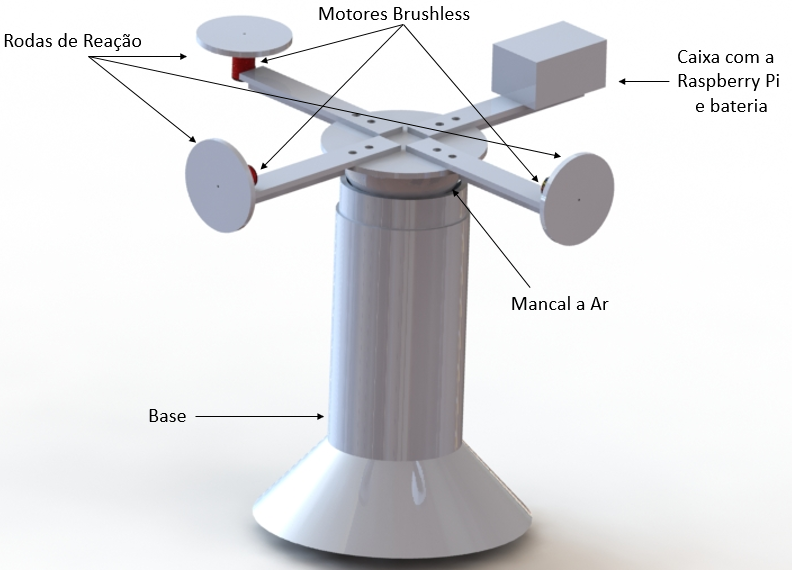
\includegraphics[scale=.75]{img/satelite_completo}
  \end{center}
  \fonte{Elaborado pelo Autor.} 
  \label{fig:satelite_completo}
\end{figure}


%%%%%%%%%%%%%%%%%%%%%%%%%%%%%%%%%%%
\subsection{Modelagem Motor DC e Rodas de Reação}

\begin{figure}[H]
  \caption{Desenho mecânico do conjunto Motor-Roda}
  \begin{center}
      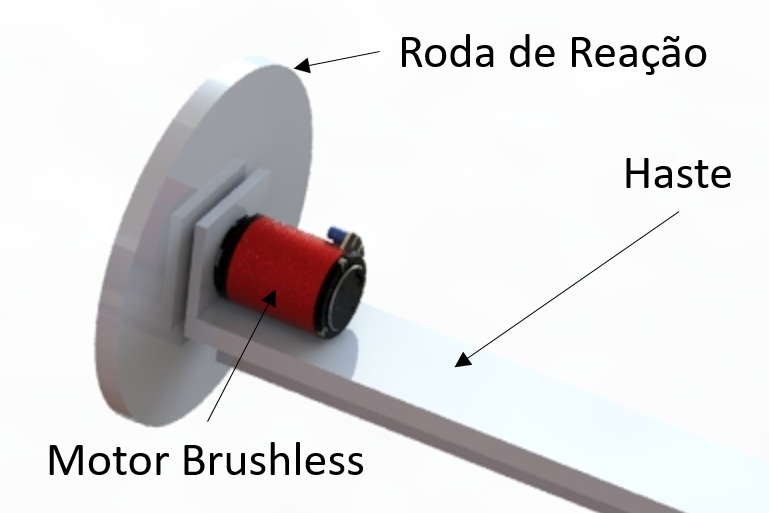
\includegraphics[scale=.45]{img/motor_roda_desenho}
  \end{center}
  \fonte{Elaborado pelo Autor.} 
  \label{fig:motor_roda_desenho}
\end{figure}


%%%%%%%%%%%%%%%%%%%%%%%%%%%%%%%%%%%
\subsection{Mancal a Ar}

\begin{figure}[H]
  \caption{Desenho Mecânico do Mancal a Ar}
  \begin{center}
      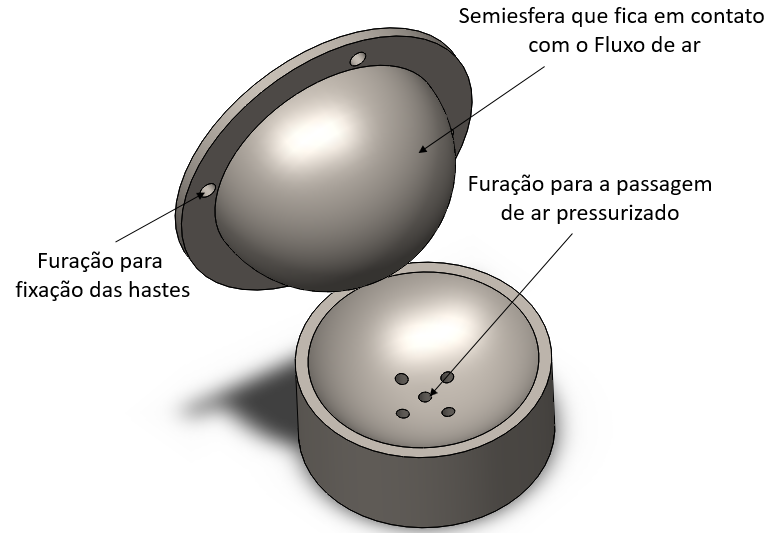
\includegraphics[scale=.45]{img/base_desenho}
  \end{center}
  \fonte{Elaborado pelo Autor.} 
  \label{fig:base_desenho}
\end{figure}

%%%%%%%%%%%%%%%%%%%%%%%%%%%%%%%%%%%
\subsection{Elementos Eletrônicos}

\begin{figure}[H]
  \caption{Raspberry Pi Zero}
  \begin{center}
      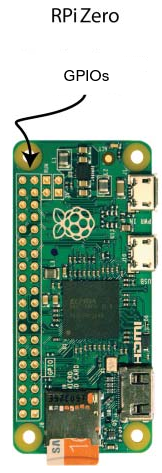
\includegraphics[scale=.55]{img/rasp_zero}
  \end{center}
  \fonte{Adaptado de \citeonline{Molloy2016}} 
  \label{fig:rasp_zero}
\end{figure}


\begin{figure}[H]
  \caption{Circuito impresso com o acelerômetro MMA7260QT}
  \begin{center}
      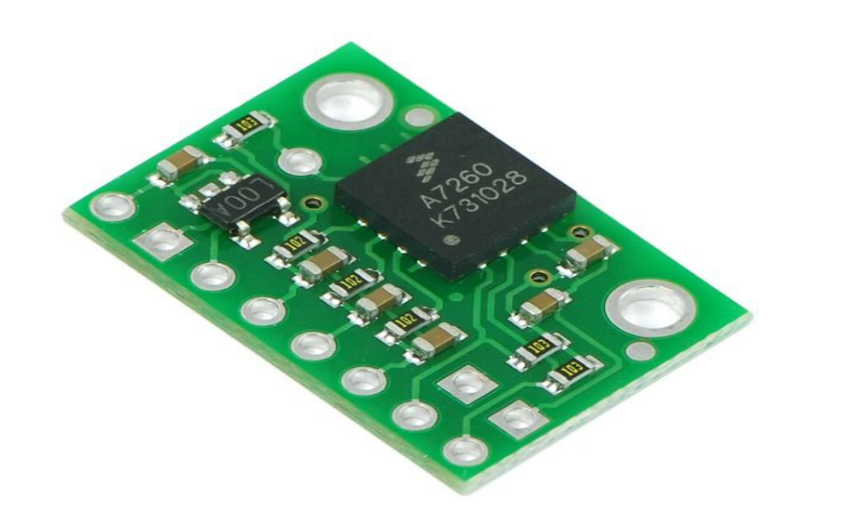
\includegraphics[scale=.4]{img/pci_acelerometro_calache_p22}
  \end{center}
  \fonte{Calache, Danilo Carreiro} 
  \label{fig:pci_acelerometro_calache_p22}
\end{figure}

%%%%%%%%%%%%%%%%%%%%%%%%%%%%%%%%%%%
\section{Sistemas de Controle}

\subsection{Modelo Motor DC}
\begin{figure}[H]
  \caption{Modelo do Motor DC}
  \begin{center}
      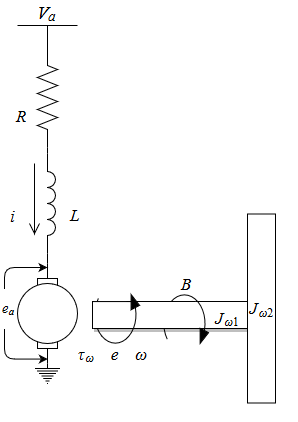
\includegraphics[scale=.65]{img/modelo_motor_dc}
  \end{center}
  \fonte{Elaborado pelo Autor.} 
  \label{fig:modelo_motor_dc}
\end{figure}

\begin{equation}
L_a \frac{di_a}{dt}+R_a i_a + e_b = e_a
\end{equation}

\begin{equation}
L_a \frac{di_a}{dt}+R_a i_a + K_2\frac{\theta}{dt} = K_1e_v
\end{equation}

\begin{equation}
\tau_{\omega} = (J_{\omega 1} + J_{\omega 2})\frac{d^{2}\theta}{dt^{2}}+B\frac{d\theta}{dt} = k_2 i_a
\end{equation}


\subsection{Modelo Completo do Satélite}

\begin{figure}[H]
  \caption{Modelo em malha aberta}
  \begin{center}
      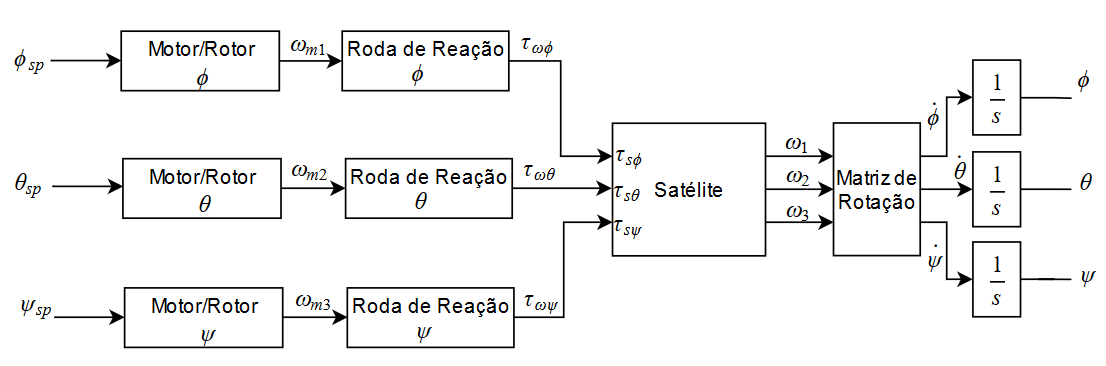
\includegraphics[scale=.55]{img/modelo_satelite_malha_aberta}
  \end{center}
  \fonte{Elaborado pelo Autor.} 
  \label{fig:modelo_satelite_malha_aberta}
\end{figure}


\begin{figure}[H]
  \caption{Modelo em malha fechada com um Controlador PID}
  \begin{center}
      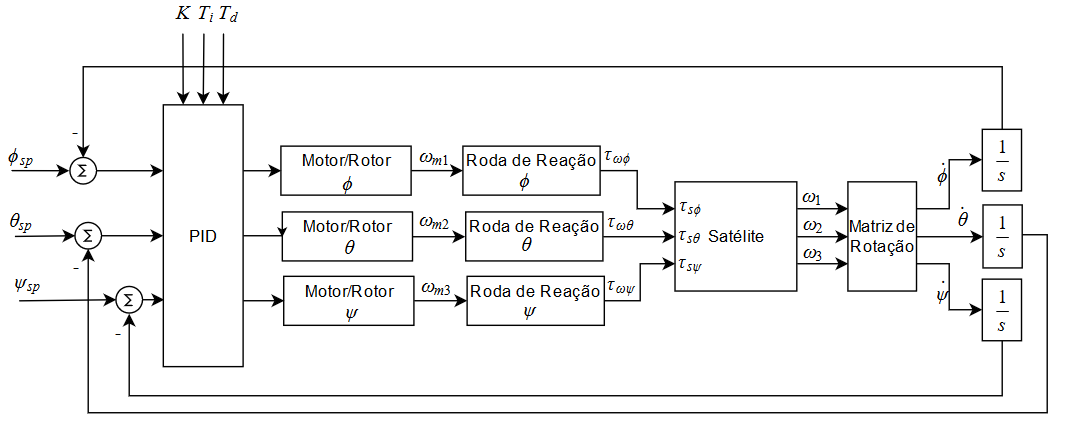
\includegraphics[scale=.55]{img/modelo_satelite_pid}
  \end{center}
  \fonte{Elaborado pelo Autor.} 
  \label{fig:modelo_satelite_pid}
\end{figure}


%%%%%%%%%%%%%%%%%%%%%%%%%%%%%%%%%%%%%%%%%%%%%%%%%%%%%%%%%%%%%%%%%%%%%%
\section{Software}

\begin{figure}[H]
  \caption{Topologia de Rede}
  \begin{center}
      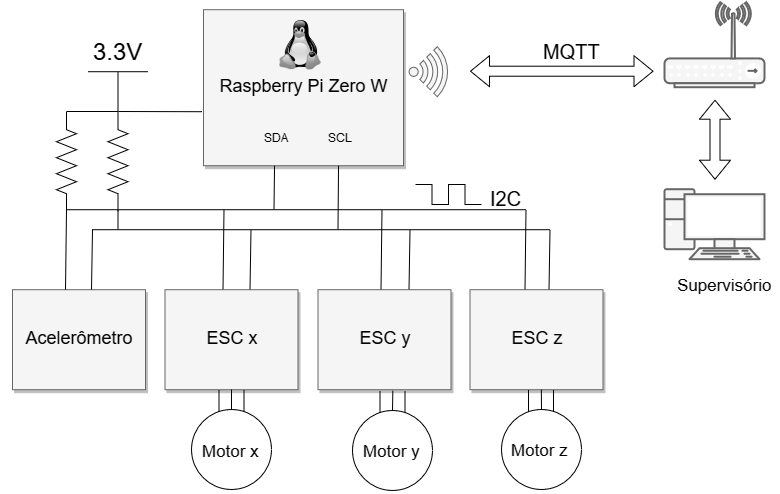
\includegraphics[scale=.75]{img/comunicacao_projeto}
  \end{center}
  \fonte{Elaborado pelo Autor.} 
  \label{fig:comunicacao_projeto}
\end{figure}

%%%%%%%%%%%%%%%%%%%%%%%%%%%%%%%%%%%
\subsection{Implementação do Controlador PID}

%%%%%%%%%%%%%%%%%%%%%%%%%%%%%%%%%%%
\subsection{Implementação da Rede Neural}

%%%%%%%%%%%%%%%%%%%%%%%%%%%%%%%%%%%
\subsection{Protocolos de Comunicação}

%%%%%%%%%%%%%%%%%%%%%%%%%%%%%%%%%%%
\subsection{Sistemas Supervisórios}
